\documentclass{beamer}

\usepackage{graphicx}
\usepackage{tikz}
\usepackage{multimedia}
\usepackage{fontspec}
\usepackage{ulem}

\RequirePackage{luatex85}


\setsansfont{texgyreheros}[
  Scale=MatchUppercase,% or MatchUppercase
  Extension=.otf,
  UprightFont=*-regular,
  ItalicFont=*-italic,
  BoldFont=*-bold,
  BoldItalicFont=*-bolditalic,
]

\defaultfontfeatures{Mapping=tex-text}

\setbeamerfont{frametitle}{family=\fontspec{Linux Biolinum}}

% Default theme as a base
\usetheme{default}

\definecolor{rr}{RGB}{56,200,0}
\definecolor{pp}{RGB}{101,42,138}
\definecolor{pr}{RGB}{0,161,255}
\definecolor{rp}{RGB}{255,39,39}

% Font
%\renewcommand\sfdefault{phv}
%\renewcommand\familydefault{\sfdefault}
%\setbeamerfont{title}{size=\Large}
%\setbeamerfont{frametitle}{size=\large}
%\setbeamercolor{frametitle}{bg=, fg=blue!70!black}
%\setbeamercolor{title}{bg=, fg=blue!70!black}
%\setbeamercolor{normal text}{bg=white, fg=black}

%\setbeamertemplate{footline}[frame number]

% Structure
\setbeamertemplate{itemize items}[default]
\setbeamertemplate{enumerate items}[circle]

%\setbeamertemplate{itemize item}[triangle]
\setbeamertemplate{itemize subitem}[circle]
\setbeamercolor{structure}{fg=black}
\setbeamercolor{item}{fg=RoyalBlue}
\setbeamercolor{itemize item}{fg=black}
\setbeamercolor{itemize subitem}{fg=black}
\setbeamercolor{itemize subsubitem}{fg=black}

\setbeamersize{text margin left=.5cm,text margin right=.5cm} 

% Features
\setbeamertemplate{headline}{}
\setbeamertemplate{navigation symbols}{}
%\setbeamertemplate{footline}{}

%\setbeamercolor{section in head/foot}{use=structure,bg=Blue!15!bg}
%\AtBeginDocument{%
%  {\usebeamercolor{section in head/foot}}
%  \pgfdeclareverticalshading{beamer@headfade}{\paperwidth}{%
%    color(0.0cm)=(bg); color(1.5cm)=(section in head/foot.bg) }
%  \setbeamercolor{section in head/foot}{bg=}
%}
%\addtoheadtemplate{\pgfuseshading{beamer@headfade}\vskip-1.5cm}{}

\newcommand{\mb}[1]{\mathbf{#1}}
\newcommand{\bs}[1]{\boldsymbol{#1}}
\newcommand{\gr}[1]{{\tiny\color{green!50!black} #1}}
\newcommand{\grb}[1]{{\small\color{green!50!black} #1}}
\newcommand{\cb}[1]{{\color{blue} #1}}
\newcommand{\crr}[1]{{\color{red} #1}}

\begin{document}



%{
%  \usebackgroundtemplate{\includegraphics[width=\paperwidth]{oesper_title.pdf}}
%\begin{frame}
%
%\end{frame}
%}

\begin{frame}{Shortcuts to adiabaticity}

  \begin{figure}
\includegraphics<1>[width=\textwidth]{analogy1.pdf}\includegraphics<2>[width=\textwidth]{analogy2.pdf}\includegraphics<3>[width=\textwidth]{analogy3.pdf}
  \end{figure}

\end{frame}

\begin{frame}{Traditional view of protein production}

  \begin{figure}
    \includegraphics<1>[width=\textwidth]{dogma1.pdf}\includegraphics<2>[width=\textwidth]{dogma1b.pdf}\includegraphics<3>[width=\textwidth]{dogma2.pdf}
  \end{figure}
  
\end{frame}

\begin{frame}{Proteins function at the cliff edge of unfolding}

  \begin{columns}
    \column{0.5\textwidth}
  \begin{figure}
    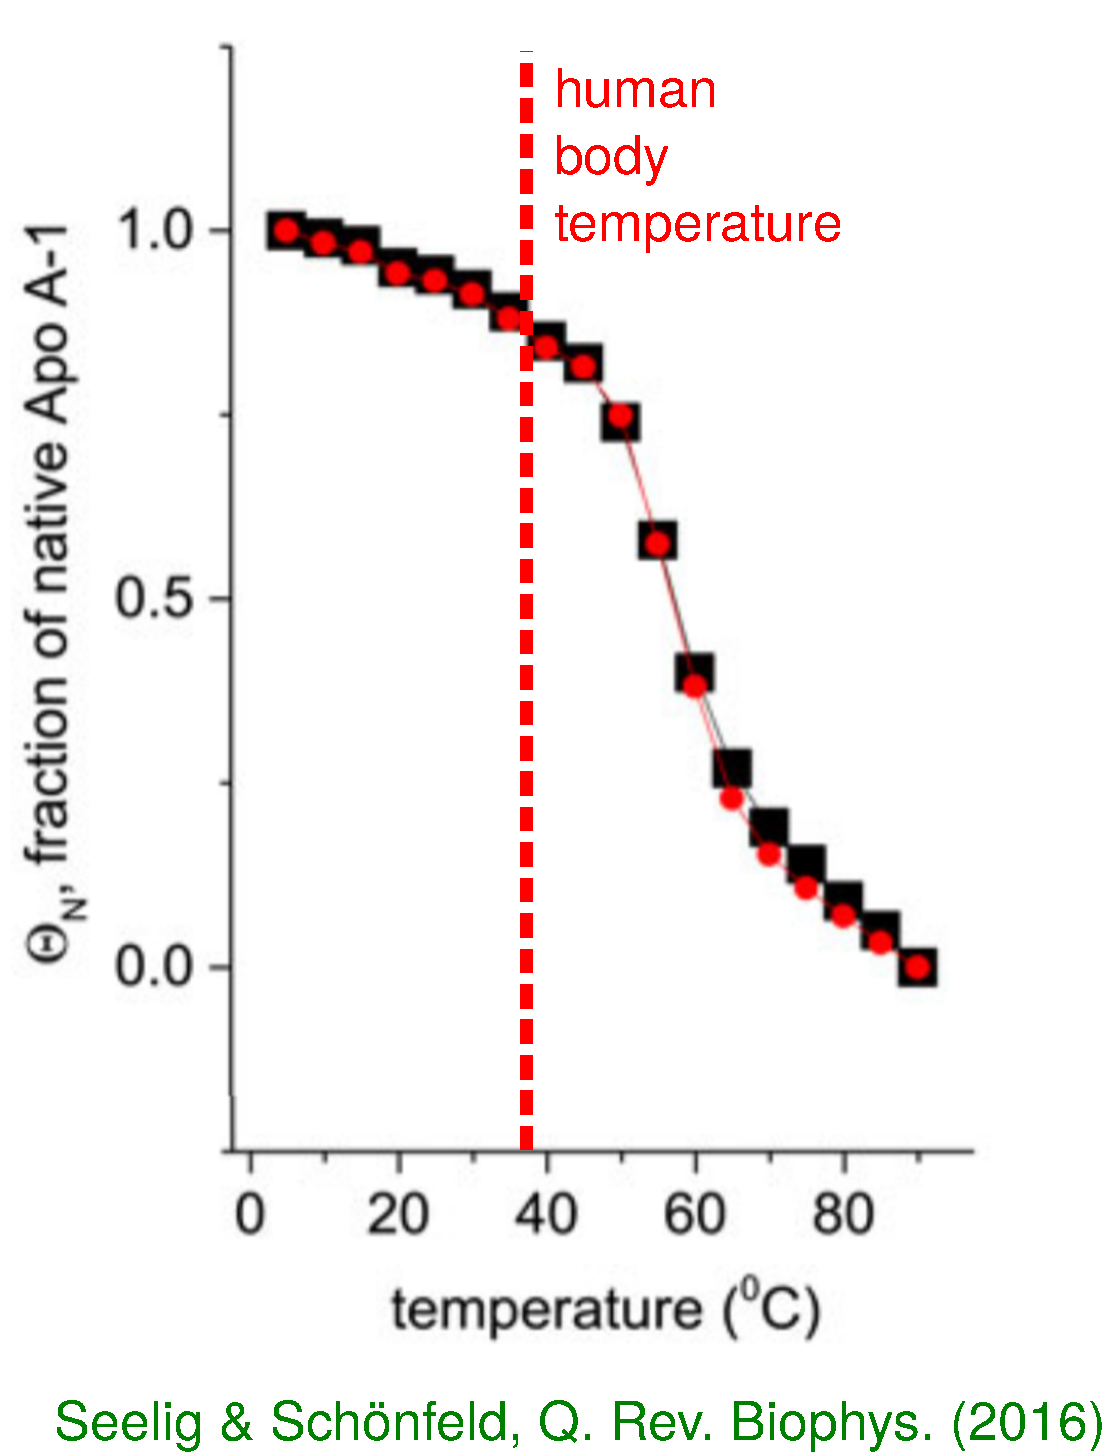
\includegraphics[width=\textwidth]{thermal_unfold.pdf}
  \end{figure}

  \pause
  \column{0.45\textwidth} Being on the verge of melting gives proteins
  the {\color{blue}dynamical flexibility} essential for their diverse roles as enzymes.

  \pause

  \vspace{1em}
  
  But it also makes them highly vulnerable to changes in temperature
  (even of a few degrees):  {\color{red} heat shock}.
  \end{columns}
\end{frame}

\begin{frame}{The protein ``hospital'':  possible chaperone pathways}
  \vspace{0.5em}
  \begin{figure}
\centering    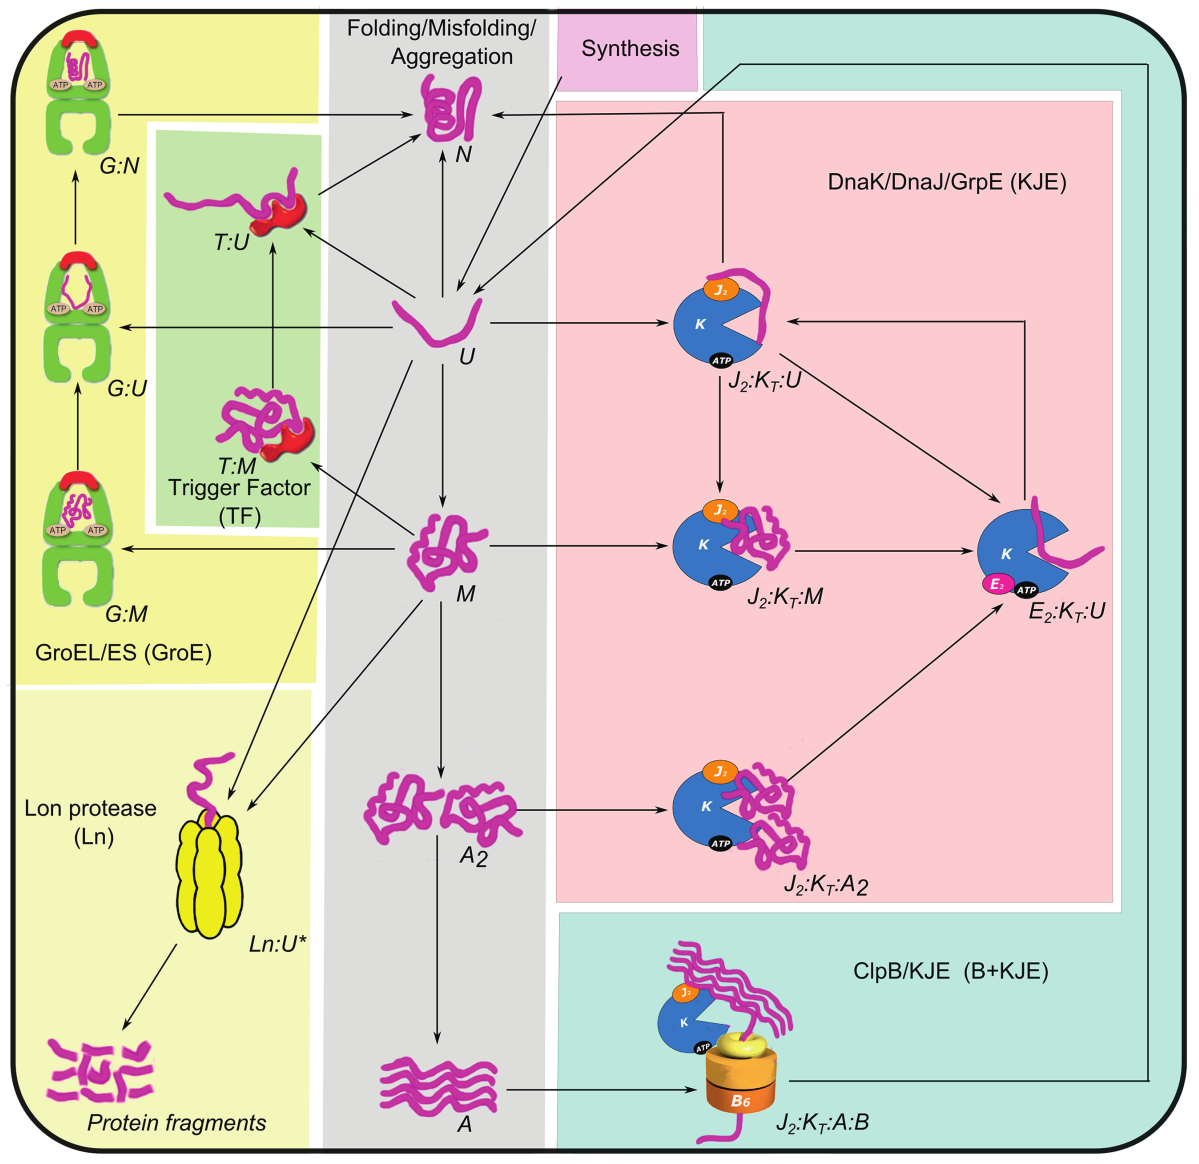
\includegraphics[width=0.65\textwidth]{ecoli_network.png}\\
      {{\it E. coli} chaperone network: \color{green!50!black}Santra {\it et al.}, PNAS (2017)}
  \end{figure}
\end{frame}

\begin{frame}{The protein ``hospital'':  possible chaperone pathways}

  \vspace{0.5em} Different classes of proteins interact primarily with
  different chaperone sub-systems:
  \begin{figure}
    \centering
    \includegraphics<1>[width=\textwidth]{ecoli_flux1.png}\includegraphics<2>[width=\textwidth]{ecoli_flux2.png}\includegraphics<3>[width=\textwidth]{ecoli_flux3.png}\\[1em]
 {\color{green!50!black}Santra {\it et al.}, PNAS (2017)}
  \end{figure}

  \pause\pause
      {\color{red} Under optimal growth conditions, chaperones are nearly fully occupied by ``patient'' proteins:  spare capacity is too energetically costly.}
  
\end{frame}


\begin{frame}{Example: heat shock response in yeast}

  \vspace{1em}
  \begin{figure}
    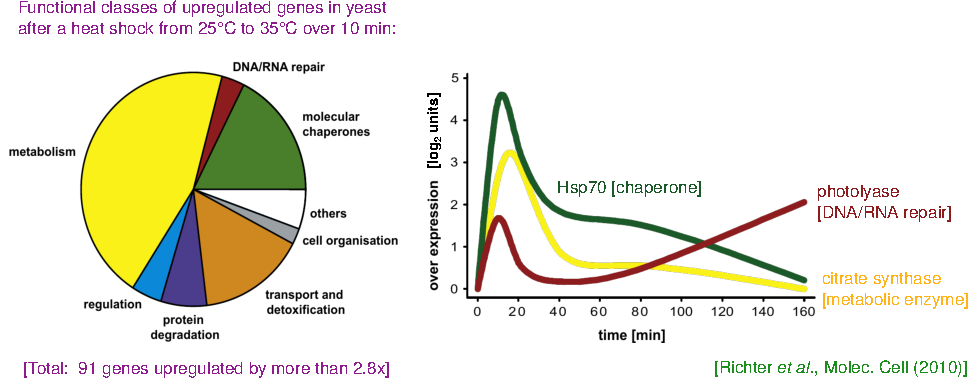
\includegraphics[width=\textwidth]{yeast_response.pdf}
  \end{figure}
\end{frame}

\end{document}

